\section{Introducción}

En este trabajo práctico se desarrolla una herramienta para realizar un \textit{traceroute}, el cual permite detectar las rutas que atraviezan los paquetes a lo largo de Internet para viajar de un punto a otro en la que se obtienen las direcciones IP de los saltos junto a sus respectivos RTTs (Round Trip Time).

Con este fin se decidió hacer uso del protocolo ICMP (\textit{Internet Control Message Protocol}) en el cual se basan algunas implementaciones de traceroute.\\

El protocolo ICMP tiene como objetivo brindar mensajes de control dentro de una comunicación\cite{ICMP}. Utiliza de soporte a IP y debería ser impelmentado por todo módulo IP. No hay garantía que el datagrama o el mensaje de control llegue a destino. Los mensajes ICMP se envían a la dirección fuente del datagrama IP que generó el mensaje y ningun mensaje ICMP reporta a otro mensaje ICMP. Una de los motivos más comunes de intercambio de estos paquetes ICMP se deben a que el destino no puede ser alcanzado, o a que el TTL (Time To Live) asociado al paquete IP en el cual se monta llega a cero.\\

Un paquete que utiliza el protocolo ICMP posee un header de 8 bytes y una porción de datos de tamaño variable. El header cuenta con los siguientes campos: 

\begin{itemize}
\item \textbf{Tipo:} Campo de 1 byte que especifica el tipo de mensaje ICMP. Ej: Echo request.
\item \textbf{Código:} Campo de 1 byte que especifica el subtipo.
\item \textbf{Checksum:} Para control de errores. 2 Bytes.
\item \textbf{Parámetros:} OCupan 4 bytes y dependen del campo tipo.
\end{itemize}

\begin{figure}[H]
\centering
\caption{Forma del paquete ICMP}
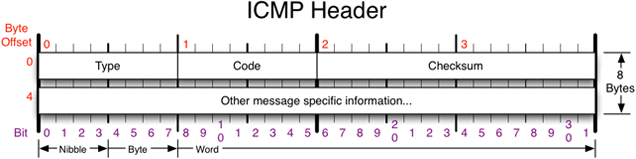
\includegraphics[width=0.55\textwidth]{modules/ICMP-Header.png}
 \label{fig:Header_ICMP}
\end{figure}

En el presente trabajo se hace uso unicamente de los tipos de mensaje \textit{Echo Request},\textit{Time Exceeded} y \textit{Echo Reply} (tipo 8,0 y 11). El primer tipo es el que se encapsula en el paquete ICMP proveniente del host que originalmente envía el pedido. El segundo puede provocarse cuando el TTL del paquete expire. Por último, \textit{Echo Reply} es la respuesta del host destino al originario del pedido Echo. En caso de que no se pueda acceder a destino, se envía Destination Unreachable.\\
 De esta manera se provee un mecanismo para corroborar la comunicación entre dos hosts. A su vez, cada respuesta calcula el RTT entre el router que responde y el host. En esta información se apoya la estimación de saltos intercontinentales mediante el análisis estadístico de la misma.
